\documentclass[10pt,a4paper]{article}
\usepackage[a4paper,top=19mm,bottom=18mm,left=20mm,right=20mm,footskip=9mm]{geometry}
\usepackage{fontspec,xcolor,tikz,tcolorbox,tabularx,booktabs,enumitem,fancyhdr,microtype}
\usepackage{graphicx}
\special{dvipdfmx:config z 0}   % ohne Kompression, maximale Druckkompatibilitaet
\usetikzlibrary{arrows.meta,shadows.blur,fit}
\tcbuselibrary{skins}
\usepackage[ngerman,provide=*]{babel}
% Trennmuster wie beim Original-Build (dort fehlten die deutschen Muster,
% babel nahm die englischen). Ohne diese Zeile bricht Seite 5 anders um.
\babelprovide[hyphenrules=english]{ngerman}
\usepackage{hyperref}\hypersetup{hidelinks,pdftitle={Kontogrundlagen & Kosten – Schulungseinheit},pdfsubject={Balance, Equity, Margin, Free Margin, Leverage, Swap}}

\setmainfont{IBMPlexSans-Regular.otf}[Path=../../fonts/,
  BoldFont={IBMPlexSans-SemiBold.otf}, ItalicFont={IBMPlexSans-Italic.otf},
  BoldItalicFont={IBMPlexSans-SemiBoldItalic.otf}]
\newfontfamily\light{IBMPlexSans-Light.otf}[Path=../../fonts/,
  BoldFont={IBMPlexSans-Regular.otf}, ItalicFont={IBMPlexSans-LightItalic.otf}]
\newfontfamily\mono{IBMPlexMono-Regular.otf}[Path=../../fonts/,
  BoldFont={IBMPlexMono-SemiBold.otf}]
\newcommand{\num}[1]{{\mono #1}}

% ---- Farben -------------------------------------------------------------
\definecolor{ink}{HTML}{14161A}    \definecolor{body}{HTML}{3C4249}
\definecolor{muted}{HTML}{6D757E}  \definecolor{soft}{HTML}{9AA1AA}
\definecolor{rule}{HTML}{E2E5E9}   \definecolor{greya}{HTML}{A8AEB6}
\definecolor{buy}{HTML}{0E7A4E}    \definecolor{sell}{HTML}{B23A2E}
\definecolor{buytint}{HTML}{E9F4EE} \definecolor{selltint}{HTML}{FAEDEB}
\definecolor{paper}{HTML}{F7F8F9}
% Farbrollen wie im Pending-Orders-Guide, keine eigene Akzentfarbe (nur Grafiken und Kaesten,
% nicht Text und nicht die Plattform-Nachbauten):
%   pfgrau  gebundene Flaechen (Margin) wie die grauen Kerzen der Charts; Text darauf ink
%   greya   Rand weisser Flaechen (Free, Volumen, Kaesten) und Hilfslinien
%   buy/sell mit buytint/selltint  Gewinn/Verlust; Strichelung in der Order-Farbe wie TP-Linien
%   pfgrey  Verlaufslinie wie die Kurslinie; ink nur als kleiner Akzent (Titellinie,
%           Merk-Kante, Punkte, Nummernkreise); paper nur im Merk-Kasten; rule Trennlinien
\definecolor{pfbg}{HTML}{001328}\definecolor{pfgruen}{HTML}{0E7A4E}
\definecolor{pfgrau}{HTML}{97A5B4}\definecolor{pfrot}{HTML}{B23A2E}
\definecolor{pfgrey}{HTML}{6A6A6A}
\definecolor{wbg}{HTML}{0E2939} \definecolor{whead}{HTML}{0B2130} \definecolor{wfield}{HTML}{102B3C}
\definecolor{wborder}{HTML}{1D4256} \definecolor{waccent}{HTML}{1B6CA8} \definecolor{wgreen}{HTML}{3CB44A}
\definecolor{wtext}{HTML}{E7EEF2} \definecolor{wmuted}{HTML}{8FA6B3} \definecolor{wmark}{HTML}{3F88BD}
\definecolor{wdim}{HTML}{5F7A89} \definecolor{wtog}{HTML}{33505F} \definecolor{wknob}{HTML}{C3D2DA}
\definecolor{wred}{HTML}{E0524D} \definecolor{wchart}{HTML}{0B2030} \definecolor{wpill}{HTML}{5B6B76}
\definecolor{wtabtext}{HTML}{CDDBE3} \definecolor{wbadge}{HTML}{0B3A17}

% ---- Typografische Skala (1,25) -----------------------------------------
\newcommand{\display}{\light\fontsize{30}{34}\selectfont}
\newcommand{\hone}{\fontsize{19}{23}\selectfont\bfseries}
\newcommand{\htwo}{\fontsize{8}{11}\selectfont\bfseries}
\newcommand{\hthree}{\fontsize{12}{15}\selectfont\bfseries}
\newcommand{\leadf}{\light\fontsize{11.5}{17}\selectfont}
\renewcommand{\small}{\fontsize{8.6}{12.4}\selectfont}
\newcommand{\lbl}{\fontsize{7.6}{10}\selectfont}
\newcommand{\micro}{\fontsize{7}{9}\selectfont}
\newcommand{\wfont}{\fontsize{6.8}{8}\selectfont}
\newcommand{\wsmall}{\fontsize{5.8}{7}\selectfont}
\newcommand{\fine}{\fontsize{7.4}{9.2}\selectfont}
\newcommand{\foot}{\fontsize{6.2}{7.6}\selectfont}
\newcommand{\ls}{\addfontfeatures{LetterSpace=14}}
\newcommand{\lsx}{\addfontfeatures{LetterSpace=8}}
\normalsize\fontsize{9.4}{14}\selectfont
\color{body}\setlength{\parindent}{0pt}\setlength{\parskip}{0pt}
\setlength{\emergencystretch}{2em}
\hyphenpenalty=400\relax

% ---- Bausteine ----------------------------------------------------------
\newcommand{\kicker}[2]{{\htwo\ls\color{muted}\MakeUppercase{#2}\par}%
  \vspace{2mm}{\color{rule}\rule{\linewidth}{0.4pt}}\par\vspace{5.5mm}}
\newcommand{\Hone}[1]{{\hone\color{ink}#1\par}\vspace{3.5mm}}
\newcommand{\Htwo}[1]{{\htwo\ls\color{muted}\MakeUppercase{#1}\par}\vspace{4mm}}
\newcommand{\lead}[1]{{\leadf\color{body}\raggedright #1\par}}
\newcommand{\hr}{\par\vspace{7mm}{\color{rule}\rule{\linewidth}{0.4pt}}\par\vspace{6mm}}
\newcommand{\hd}[1]{{\micro\bfseries\ls\color{soft}\MakeUppercase{#1}}}
\tikzset{cnum/.style={circle,fill=ink,text=white,inner sep=0,minimum size=3.2mm,
  font=\bfseries\fontsize{5.6}{6}\selectfont}}
\newcommand{\cn}[1]{\tikz[baseline=-0.65ex]\node[cnum]{#1};}
\tikzset{pfnum/.style={circle,fill=ink,text=white,inner sep=0,minimum size=13,
  font=\bfseries\fontsize{7}{8}\selectfont}}
\newcommand{\pflab}{\fontsize{7}{8.5}\selectfont}
\newcommand{\pfn}[1]{\tikz[baseline=-0.7ex]\node[circle,fill=ink,text=white,inner sep=0,
  minimum size=4.4mm,font=\bfseries\fontsize{7}{8}\selectfont]{#1};}
\usetikzlibrary{calc,decorations.pathreplacing}
% Masslinien wie in einer technischen Zeichnung (Haarlinie greya, Stealth-Spitzen wie die
% Pfeile im Pending-Orders-Guide); die Beschriftung unterbricht die Linie wie "Kurs jetzt".
\tikzset{masspfeil/.style={line width=0.4pt,
    {Stealth[length=1.5mm,width=1.1mm]}-{Stealth[length=1.5mm,width=1.1mm]}},
  hilfslinie/.style={greya,line width=0.3pt},
  zone/.style={line width=1.5pt,dash pattern=on 7pt off 4pt}}
\newcommand{\masslinie}[4][greya]{\draw[#1,masspfeil] (#2,#4) -- (#3,#4);}
\newcommand{\mass}[5][greya]{\masslinie[#1]{#2}{#3}{#4}%
  \node[inner sep=0,inner xsep=1.2mm,fill=white] at ({(#2+#3)/2},#4) {#5\strut};}

% weicher Schatten fuer eingebundene Grafiken
\tikzset{softshadow/.style={blur shadow={shadow blur steps=16,shadow xshift=0pt,
  shadow yshift=-0.9pt,shadow opacity=30,shadow blur radius=1.5mm}}}
\newcommand{\shadowfig}[2][80mm]{%
  \tikz[baseline=(current bounding box.north)]\node[inner sep=0,softshadow]
    {\includegraphics[width=#1]{#2}};}

\newtcolorbox{merk}{enhanced,colback=paper,colframe=paper,boxrule=0pt,arc=0pt,
  borderline west={2pt}{0pt}{ink},left=5mm,right=5mm,top=3.5mm,bottom=3.5mm,boxsep=0pt,
  before skip=6mm,after skip=0pt,fontupper=\small\color{body}}
\newtcolorbox{prule}[1]{enhanced,colback=white,colframe=rule,boxrule=0.4pt,arc=1mm,
  borderline west={2pt}{0pt}{#1},left=4mm,right=4mm,top=2.6mm,bottom=2.6mm,boxsep=0pt,
  before skip=2.2mm,after skip=0pt,fontupper=\small\color{body}}
\newtcolorbox{soft}[1][]{enhanced,colback=paper,colframe=paper,boxrule=0pt,arc=1.5mm,
  left=5mm,right=5mm,top=4mm,bottom=4mm,boxsep=0pt,before skip=0pt,after skip=0pt,
  before upper={\raggedright\hyphenpenalty=10000\relax\exhyphenpenalty=10000\relax},#1}

\pagestyle{fancy}\fancyhf{}\renewcommand{\headrulewidth}{0pt}

\fancyfoot[L]{\micro\color{soft}\ls KONTOGRUNDLAGEN \& KOSTEN · SCHULUNGSEINHEIT}
\begin{document}
\thispagestyle{empty}
{\htwo\ls\color{muted}SCHULUNGSEINHEIT}\par\vspace{11mm}
{\display\color{ink}Kontogrundlagen \& Kosten}\par\vspace{7mm}
{\color{ink}\rule{28mm}{2pt}}\par\vspace{6mm}
\begin{minipage}{126mm}\lead{Diese Schulungseinheit erläutert die Begriffe Balance, Equity, Margin,
Free, Level, Leverage und Swap sowie ihren Zusammenhang innerhalb Ihres Kontos.}\end{minipage}
\par\vspace{6mm}
\tikz\node[draw=rule,line width=0.4pt,rounded corners=1.6mm,inner xsep=3mm,inner ysep=1.5mm,
  text=muted,font=\micro\bfseries\ls]{KONTOWERTE UND KOSTEN};
\par\vspace{0pt plus 1fill}
\noindent 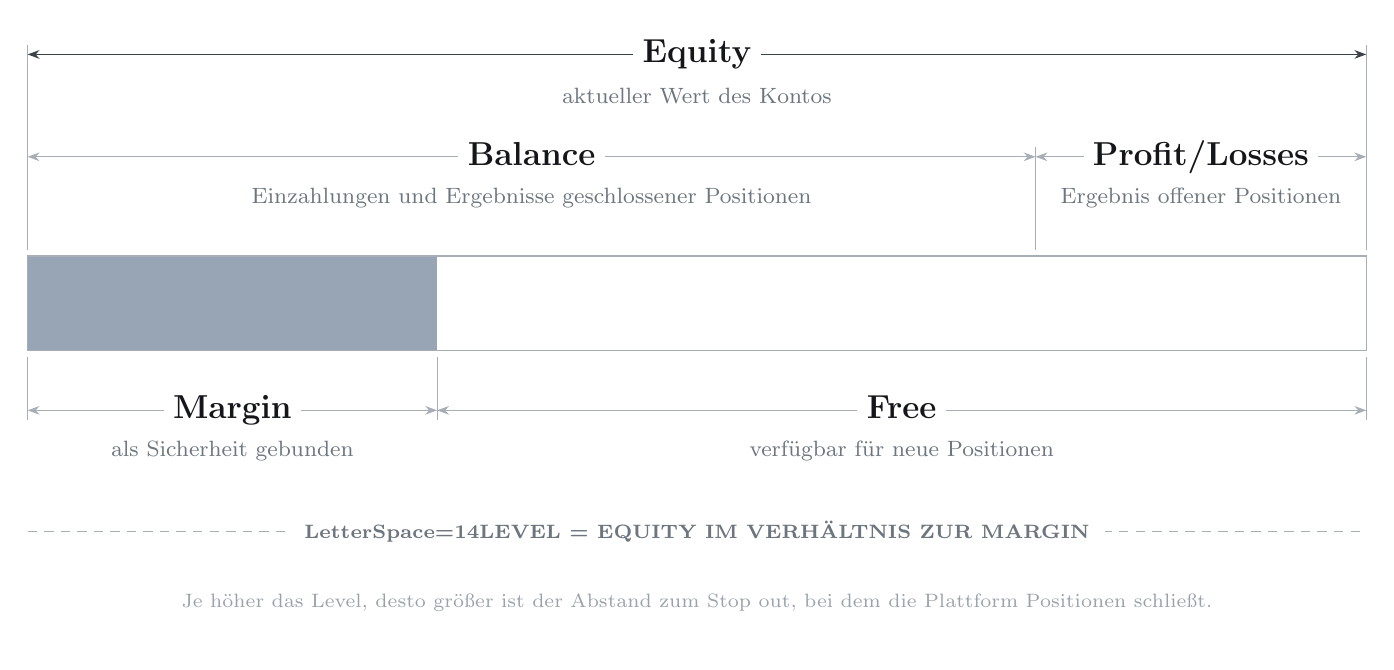
\begin{tikzpicture}[x=1mm,y=1mm]
\useasboundingbox (0,0) rectangle (170.0,78);
% Equity als ein Mengenbalken; Massketten oben (Balance + Profit/Losses) und unten
% (Margin + Free); Beschriftung unterbricht die Linie wie "Kurs jetzt" im Guide
\fill[pfgrau] (0,37) rectangle (52,49);
\draw[greya,line width=0.4pt] (0,37) rectangle (170,49);
\draw[hilfslinie] (0,49.8) -- (0,75.8) (170,49.8) -- (170,75.8) (128,49.8) -- (128,62.8)
  (0,36.2) -- (0,28.2) (52,36.2) -- (52,28.2) (170,36.2) -- (170,28.2);
\mass[body]{0}{170}{74.6}{\hthree\color{ink}Equity}
\node[inner sep=0,text=muted,font=\lbl] at (85,69.4) {aktueller Wert des Kontos};
\mass{0}{128}{61.6}{\hthree\color{ink}Balance}
\node[inner sep=0,text=muted,font=\lbl] at (64,56.4) {Einzahlungen und Ergebnisse geschlossener Positionen};
\mass{128}{170}{61.6}{\hthree\color{ink}Profit/Losses}
\node[inner sep=0,text=muted,font=\lbl] at (149,56.4) {Ergebnis offener Positionen};
\mass{0}{52}{29.4}{\hthree\color{ink}Margin}
\node[inner sep=0,text=muted,font=\lbl] at (26,24.2) {als Sicherheit gebunden};
\mass{52}{170}{29.4}{\hthree\color{ink}Free}
\node[inner sep=0,text=muted,font=\lbl] at (111,24.2) {verfügbar für neue Positionen};
\draw[greya,line width=0.5pt,dash pattern=on 1.2mm off 0.9mm] (0,14) -- (170,14);
\node[inner sep=0,fill=white,inner xsep=2mm,text=muted,font=\micro\bfseries\ls] at (85,14) {LEVEL = EQUITY IM VERHÄLTNIS ZUR MARGIN};
\node[inner sep=0,text=soft,font=\micro] at (85,5) {Je höher das Level, desto größer ist der Abstand zum Stop out, bei dem die Plattform Positionen schließt.};
\end{tikzpicture}
\par\vspace{0pt plus 1.35fill}
{\color{rule}\rule{\linewidth}{0.4pt}}\par\vspace{2.5mm}
{\micro\ls\color{soft}KONTOGRUNDLAGEN \& KOSTEN\hfill SCHULUNGSEINHEIT}
\clearpage
\kicker{}{Kontostand}
\Hone{Der Unterschied zwischen Balance und Equity}
\begin{minipage}{128mm}\lead{Die Plattform weist für Ihr Konto zwei Werte aus. Die Differenz zwischen
ihnen entspricht dem aktuellen Ergebnis Ihrer offenen Positionen.}\end{minipage}
\par\vspace{8mm}
\noindent\begin{minipage}[t]{82mm}\vspace{0pt}\begin{soft}[equal height group=konto]
{\htwo\ls\color{muted}BALANCE}\par\vspace{2mm}
{\hthree\color{ink}Der realisierte Kontostand}\par\vspace{1.5mm}
{\color{body}Die Balance umfasst Ihre Einzahlungen sowie alle Gewinne und Verluste aus bereits
geschlossenen Positionen. Sie ändert sich nur, wenn Sie eine Position schließen, eine Ein- oder Auszahlung
vornehmen oder ein Swap gebucht wird.}\end{soft}\end{minipage}\hfill
\begin{minipage}[t]{82mm}\vspace{0pt}\begin{soft}[equal height group=konto]
{\htwo\ls\color{muted}EQUITY}\par\vspace{2mm}
{\hthree\color{ink}Der aktuelle Kontowert}\par\vspace{1.5mm}
{\color{body}Die Equity entspricht der Balance zuzüglich Profit/Losses, also des aktuellen Ergebnisses
Ihrer offenen Positionen. Sie verändert sich folglich mit jeder Kursbewegung. Free und Level werden auf
Grundlage dieses Werts berechnet.}\end{soft}\end{minipage}
\par\vspace{7mm}
\noindent 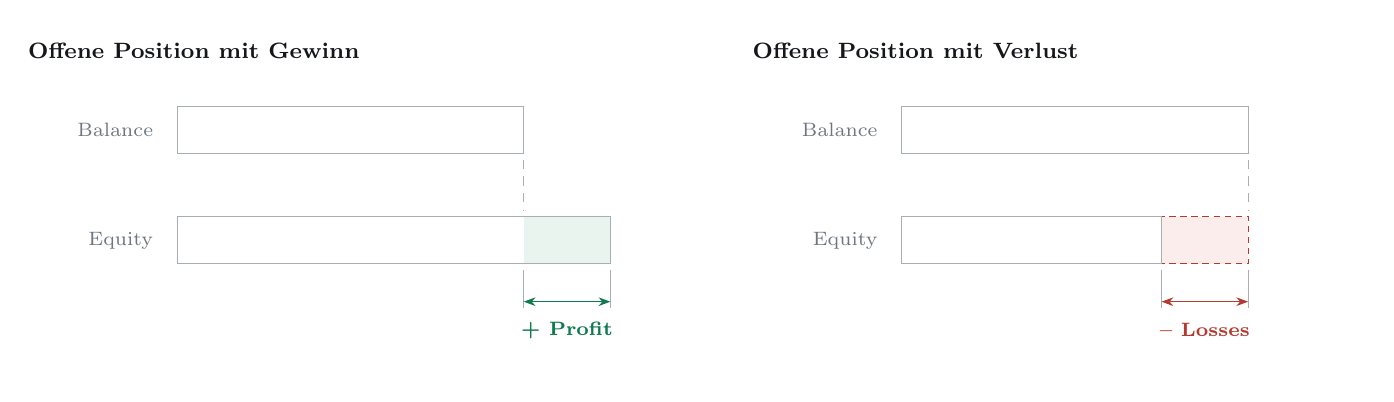
\begin{tikzpicture}[x=1mm,y=1mm]
\useasboundingbox (0,0) rectangle (170.0,44);
\node[anchor=west,inner sep=0,text=ink,font=\lbl\bfseries] at (0,41) {Offene Position mit Gewinn};
\node[anchor=east,inner sep=0,text=muted,font=\micro] at (16,31) {Balance};
\draw[greya,line width=0.4pt] (19,28) rectangle (63,34);
\node[anchor=east,inner sep=0,text=muted,font=\micro] at (16,17) {Equity};
\fill[buytint] (63,14) rectangle (74,20);
\draw[greya,line width=0.4pt] (19,14) rectangle (74,20);
\draw[greya,line width=0.4pt,dash pattern=on 1.2mm off 0.9mm] (63,27.2) -- (63,20.8);
\draw[hilfslinie] (63,13.2) -- (63,8.4) (74,13.2) -- (74,8.4);
\masslinie[buy]{63}{74}{9.2}
\node[inner sep=0,text=buy,font=\micro\bfseries] at (68.5,5.6) {+ Profit};
\node[anchor=west,inner sep=0,text=ink,font=\lbl\bfseries] at (92,41) {Offene Position mit Verlust};
\node[anchor=east,inner sep=0,text=muted,font=\micro] at (108,31) {Balance};
\draw[greya,line width=0.4pt] (111,28) rectangle (155,34);
\node[anchor=east,inner sep=0,text=muted,font=\micro] at (108,17) {Equity};
\fill[selltint] (144,14) rectangle (155,20);
\draw[sell,line width=0.4pt,dash pattern=on 0.8mm off 0.6mm] (144,14) rectangle (155,20);
\draw[greya,line width=0.4pt] (111,14) rectangle (144,20);
\draw[greya,line width=0.4pt,dash pattern=on 1.2mm off 0.9mm] (155,27.2) -- (155,20.8);
\draw[hilfslinie] (144,13.2) -- (144,8.4) (155,13.2) -- (155,8.4);
\masslinie[sell]{144}{155}{9.2}
\node[inner sep=0,text=sell,font=\micro\bfseries] at (149.5,5.6) {– Losses};
\end{tikzpicture}
\hr
\Htwo{Unrealisierte und realisierte Ergebnisse}
{\color{body}\raggedright Solange eine Position offen ist, stellt ihr Gewinn oder Verlust lediglich eine Momentaufnahme dar.
Die Plattform weist ihn unter \textbf{Profit/Losses} aus und berücksichtigt ihn in der Equity, nicht jedoch in der
Balance. Erst mit dem Schließen der Position wird der Betrag realisiert.\par}
\par\vspace{5mm}
\noindent 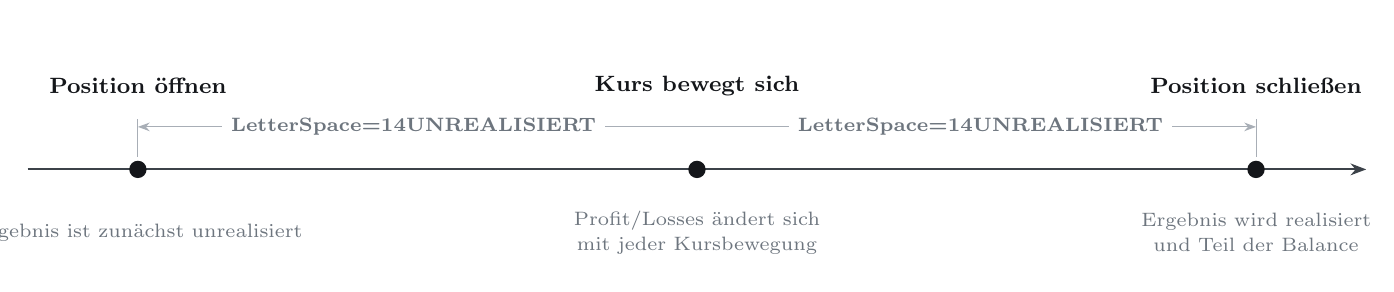
\begin{tikzpicture}[x=1mm,y=1mm]
\useasboundingbox (0,0) rectangle (170.0,30);
\draw[body,line width=0.7pt,-{Stealth[length=2mm]}] (0,12) -- (170.0,12);
\draw[hilfslinie] (14,13.6) -- (14,18.4) (156,13.6) -- (156,18.4);
\masslinie{14}{156}{17.4}
\node[inner sep=0,inner xsep=1.2mm,fill=white,text=muted,font=\micro\bfseries\ls] at (49,17.4) {UNREALISIERT};
\node[inner sep=0,inner xsep=1.2mm,fill=white,text=muted,font=\micro\bfseries\ls] at (121,17.4) {UNREALISIERT};
\fill[ink] (14,12) circle (1.1);
\node[inner sep=0,text=ink,font=\lbl\bfseries] at (14,22.6) {Position öffnen};
\node[inner sep=0,text=muted,font=\micro,text width=44mm,align=center] at (14,4) {Ergebnis ist zunächst unrealisiert};
\fill[ink] (85,12) circle (1.1);
\node[inner sep=0,text=ink,font=\lbl\bfseries] at (85,22.6) {Kurs bewegt sich};
\node[inner sep=0,text=muted,font=\micro,text width=44mm,align=center] at (85,4) {Profit/Losses ändert sich mit jeder Kursbewegung};
\fill[ink] (156,12) circle (1.1);
\node[inner sep=0,text=ink,font=\lbl\bfseries] at (156,22.6) {Position schließen};
\node[inner sep=0,text=muted,font=\micro,text width=44mm,align=center] at (156,4) {Ergebnis wird realisiert\\und Teil der Balance};
\end{tikzpicture}
\par\vspace{4mm}
\begin{merk}\textbf{Zur Einordnung.} Die Balance enthält keine Angaben zu offenen Positionen. Den aktuellen
Stand Ihres Kontos geben folglich Equity und Profit/Losses wieder.\end{merk}
\clearpage
\kicker{}{Margin}
\Hone{Die Margin als Sicherheitsleistung}
\begin{minipage}{128mm}\lead{Sobald Sie eine Position öffnen, bindet die Plattform einen Teil Ihrer Equity
als Sicherheit. Dieser Betrag wird nicht verbraucht, sondern bleibt gebunden, bis die Position geschlossen wird.}\end{minipage}
\par\vspace{8mm}
\noindent\begin{minipage}[t]{54mm}\vspace{0pt}\raggedright
{\bfseries Margin}\par\vspace{1mm}
{\color{muted}\small Der als Sicherheit gebundene Teil der Equity. Er wird in der Kontoübersicht und bei jeder Position einzeln ausgewiesen.}
\end{minipage}\hfill
\begin{minipage}[t]{54mm}\vspace{0pt}\raggedright
{\bfseries Free}\par\vspace{1mm}
{\color{muted}\small Der nicht gebundene Teil der Equity. Nur dieser Betrag steht für weitere Positionen zur Verfügung.}
\end{minipage}\hfill
\begin{minipage}[t]{54mm}\vspace{0pt}\raggedright
{\bfseries Level}\par\vspace{1mm}
{\color{muted}\small Das Verhältnis von Equity zu Margin. Es dient als Maßstab für den Abstand zum Stop out.}
\end{minipage}
\par\vspace{8mm}
\noindent 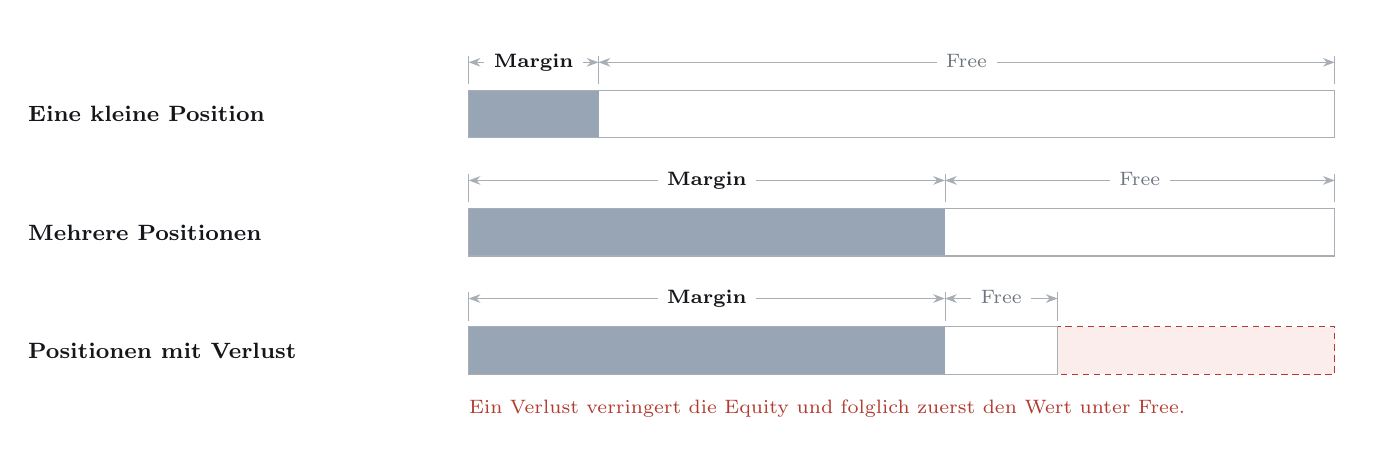
\begin{tikzpicture}[x=1mm,y=1mm]
\useasboundingbox (0,0) rectangle (170.0,50);
\node[anchor=west,inner sep=0,text=ink,font=\lbl\bfseries] at (0,39) {Eine kleine Position};
\fill[pfgrau] (56,36) rectangle (72.5,42);
\draw[greya,line width=0.4pt] (56,36) rectangle (166.0,42);
\draw[hilfslinie] (56,42.8) -- (56,46.4) (72.5,42.8) -- (72.5,46.4) (166.0,42.8) -- (166.0,46.4);
\mass{56}{72.5}{45.6}{\micro\bfseries\color{ink}Margin}
\mass{72.5}{166.0}{45.6}{\micro\color{muted}Free}
\node[anchor=west,inner sep=0,text=ink,font=\lbl\bfseries] at (0,24) {Mehrere Positionen};
\fill[pfgrau] (56,21) rectangle (116.5,27);
\draw[greya,line width=0.4pt] (56,21) rectangle (166.0,27);
\draw[hilfslinie] (56,27.8) -- (56,31.4) (116.5,27.8) -- (116.5,31.4) (166.0,27.8) -- (166.0,31.4);
\mass{56}{116.5}{30.6}{\micro\bfseries\color{ink}Margin}
\mass{116.5}{166.0}{30.6}{\micro\color{muted}Free}
\node[anchor=west,inner sep=0,text=ink,font=\lbl\bfseries] at (0,9) {Positionen mit Verlust};
\fill[pfgrau] (56,6) rectangle (116.5,12);
\fill[selltint] (130.8,6) rectangle (166.0,12);
\draw[sell,line width=0.4pt,dash pattern=on 0.8mm off 0.6mm] (130.8,6) rectangle (166.0,12);
\draw[greya,line width=0.4pt] (56,6) rectangle (130.8,12);
\draw[hilfslinie] (56,12.8) -- (56,16.4) (116.5,12.8) -- (116.5,16.4) (130.8,12.8) -- (130.8,16.4);
\mass{56}{116.5}{15.6}{\micro\bfseries\color{ink}Margin}
\mass{116.5}{130.8}{15.6}{\micro\color{muted}Free}
\node[anchor=west,inner sep=0,text=sell,font=\micro] at (56,1.6) {Ein Verlust verringert die Equity und folglich zuerst den Wert unter Free.};
\end{tikzpicture}
\par\vspace{5mm}
{\color{body}\raggedright Größere Positionen und eine höhere Anzahl an Positionen binden mehr Margin. Verluste verringern
zudem die Equity. Der Wert unter Free nimmt folglich aus zwei Gründen ab.\par}
\hr
\Htwo{Level, Warnbereich und Stop out}
{\color{body}\raggedright Solange die Equity deutlich über der gebundenen Margin liegt, ist das Level hoch. Sinkt die Equity
durch Verluste, sinkt folglich auch das Level. Ab einer bestimmten Schwelle gibt die Plattform eine Warnung aus.
Erreicht das Level den \textbf{Stop out}, schließt die Plattform Positionen selbstständig, beginnend mit der Position
mit dem größten Verlust. Den Stop-out-Wert Ihres Kontos finden Sie unter \textbf{Information}.\par}
\par\vspace{5mm}
\noindent 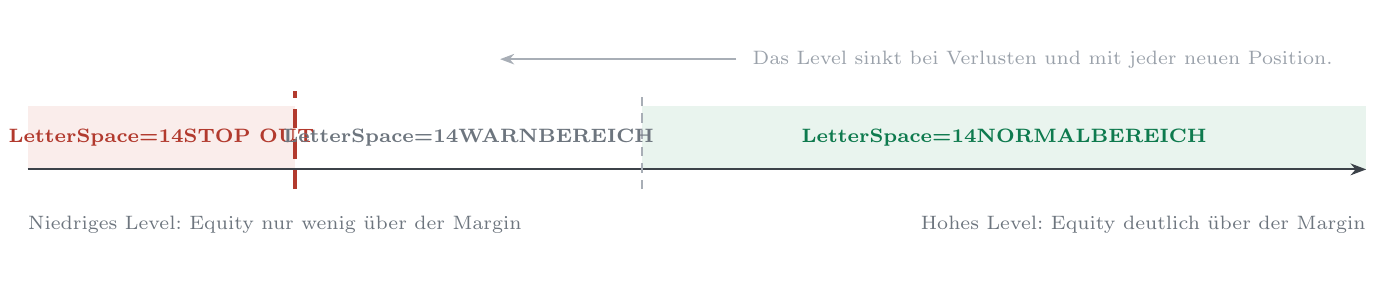
\begin{tikzpicture}[x=1mm,y=1mm]
\useasboundingbox (0,0) rectangle (170.0,30);
\fill[selltint] (0,12) rectangle (34,20);\fill[buytint] (78,12) rectangle (170.0,20);
\draw[body,line width=0.7pt,-{Stealth[length=2mm]}] (0,12) -- (170.0,12);
\draw[sell,zone] (34,9.5) -- (34,22);
\draw[greya,line width=0.5pt,dash pattern=on 1.2mm off 0.9mm] (78,9.5) -- (78,22);
\node[inner sep=0,text=sell,font=\micro\bfseries\ls] at (17,16) {STOP OUT};
\node[inner sep=0,text=muted,font=\micro\bfseries\ls] at (56,16) {WARNBEREICH};
\node[inner sep=0,text=buy,font=\micro\bfseries\ls] at (124,16) {NORMALBEREICH};
\node[anchor=west,inner sep=0,text=muted,font=\micro] at (0,5) {Niedriges Level: Equity nur wenig über der Margin};
\node[anchor=east,inner sep=0,text=muted,font=\micro] at (170.0,5) {Hohes Level: Equity deutlich über der Margin};
\draw[greya,line width=0.5pt,-{Stealth[length=1.8mm]}] (90,26) -- (60,26);
\node[anchor=west,inner sep=0,text=soft,font=\micro] at (92,26) {Das Level sinkt bei Verlusten und mit jeder neuen Position.};
\end{tikzpicture}
\clearpage
\kicker{}{Hebel}
\Hone{Die Wirkung des Hebels}
\begin{minipage}{128mm}\lead{Mit Hebel bewegen Sie am Markt ein deutlich größeres Volumen, als Sie an Margin
hinterlegen. Gewinne und Verluste werden folglich am gesamten Volumen berechnet, nicht am Einsatz.}\end{minipage}
\par\vspace{8mm}
\noindent 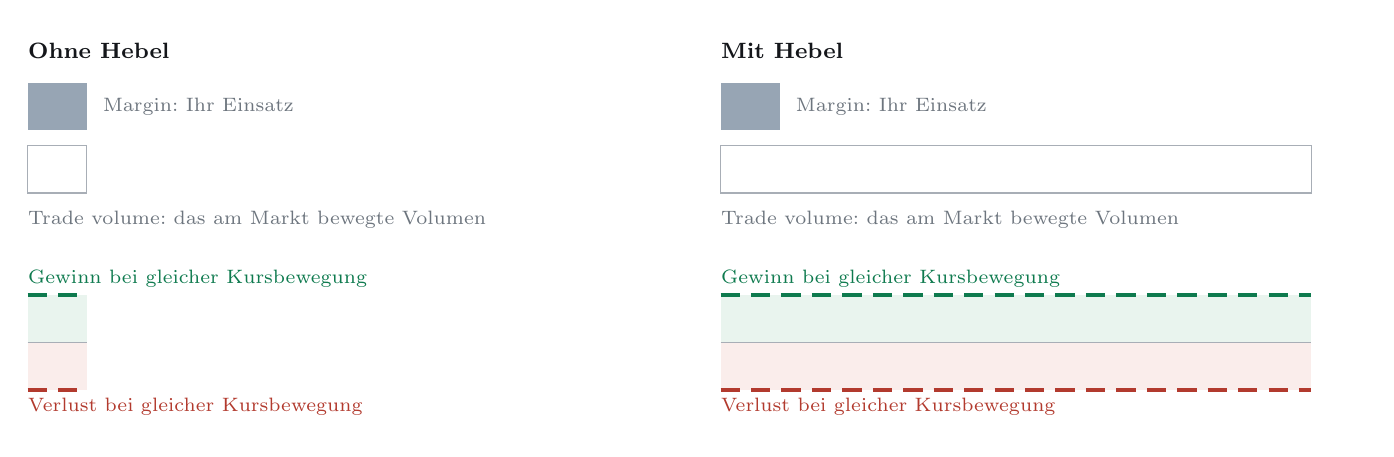
\begin{tikzpicture}[x=1mm,y=1mm]
\useasboundingbox (0,5) rectangle (170.0,56);
\node[anchor=west,inner sep=0,text=ink,font=\lbl\bfseries] at (0,53) {Ohne Hebel};
\fill[pfgrau] (0,43) rectangle (7.5,49);
\node[anchor=west,inner sep=0,text=muted,font=\micro] at (9.5,46) {Margin: Ihr Einsatz};
\draw[greya,line width=0.4pt] (0,35) rectangle (7.5,41);
\node[anchor=west,inner sep=0,text=muted,font=\micro] at (0,31.6) {Trade volume: das am Markt bewegte Volumen};
\fill[buytint] (0,16) rectangle (7.5,22);\fill[selltint] (0,10) rectangle (7.5,16);
\draw[greya,line width=0.4pt] (0,16) -- (7.5,16);
\draw[buy,zone] (0,22) -- (7.5,22);\draw[sell,zone] (0,10) -- (7.5,10);
\node[anchor=south west,inner sep=0,text=buy,font=\micro] at (0,23) {Gewinn bei gleicher Kursbewegung};
\node[anchor=north west,inner sep=0,text=sell,font=\micro] at (0,9) {Verlust bei gleicher Kursbewegung};
\node[anchor=west,inner sep=0,text=ink,font=\lbl\bfseries] at (88,53) {Mit Hebel};
\fill[pfgrau] (88,43) rectangle (95.5,49);
\node[anchor=west,inner sep=0,text=muted,font=\micro] at (97.5,46) {Margin: Ihr Einsatz};
\draw[greya,line width=0.4pt] (88,35) rectangle (163,41);
\node[anchor=west,inner sep=0,text=muted,font=\micro] at (88,31.6) {Trade volume: das am Markt bewegte Volumen};
\fill[buytint] (88,16) rectangle (163,22);\fill[selltint] (88,10) rectangle (163,16);
\draw[greya,line width=0.4pt] (88,16) -- (163,16);
\draw[buy,zone] (88,22) -- (163,22);\draw[sell,zone] (88,10) -- (163,10);
\node[anchor=south west,inner sep=0,text=buy,font=\micro] at (88,23) {Gewinn bei gleicher Kursbewegung};
\node[anchor=north west,inner sep=0,text=sell,font=\micro] at (88,9) {Verlust bei gleicher Kursbewegung};
\end{tikzpicture}
\par\vspace{6mm}
% Einzige bewusste Ausnahme vom Zahlenverbot (Nutzerwunsch, HANDOFF Abschnitt 14):
% Vergleich mit einfachen Zahlen nach dem Lehrbuchbeispiel "you vs. your friend".
% Schreibweise: 1.000\,€, 5\,%, echtes Minuszeichen U+2212.
\Htwo{Ein Vergleich mit einfachen Zahlen}
{\color{body}\raggedright Angenommen, Sie und ein Bekannter verfügen über je 100\,€ und erwarten, dass
Instrument~XY steigt. Ihr Bekannter kauft ohne Hebel und bewegt folglich genau 100\,€. Sie handeln hingegen mit Hebel~1:10:
Ihre~100\,€ sind als Margin gebunden, bewegt werden jedoch 1.000\,€. Die fehlenden 900\,€ sind geliehen.\par}
\par\vspace{4mm}
% Spalte "Mit Hebel" beginnt bei 88 mm wie "Mit Hebel" in der Grafik darueber.
\begin{tabular}{@{}>{\raggedright\arraybackslash}p{34mm}>{\raggedright\arraybackslash}p{45.53mm}%
  >{\raggedright\arraybackslash}p{82mm}@{}}
 & \hd{Ohne Hebel} & \hd{Mit Hebel 1:10} \\
\addlinespace[1.6mm]\midrule\addlinespace[2.4mm]
\textbf{Einsatz} & 100\,€ & 100\,€ als Margin \\ \addlinespace[1.6mm]
\textbf{Bewegtes Volumen} & 100\,€ & 1.000\,€ \\ \addlinespace[1.6mm]
\textbf{Kurs steigt um 5\,\%} & \textcolor{buy}{+5\,€} & \textcolor{buy}{+50\,€} \\ \addlinespace[1.6mm]
\textbf{Kurs fällt um 5\,\%} & \textcolor{sell}{−5\,€} & \textcolor{sell}{−50\,€} \\ \addlinespace[1.6mm]
\textbf{Kurs fällt um 10\,\%} & \textcolor{sell}{−10\,€} & \textcolor{sell}{−100\,€, also der gesamte Einsatz}\newline
  {\color{muted}\small Der Stop out schließt die Position in der Regel vorher.} \\ \addlinespace[1.6mm]
\textbf{Halten über Nacht} & kein Swap & Swap für die geliehenen 900\,€ \\
\end{tabular}
\par\vspace{4mm}
{\color{body}\raggedright Gemessen am Einsatz ergibt dieselbe Kursbewegung bei Ihrem Bekannten ±5\,\%, bei Ihnen hingegen
+50\,\% oder −50\,\%. Der Hebel vergrößert folglich Gewinn und Verlust im gleichen Verhältnis.\par}
\par\vspace{6mm}
\noindent\begin{minipage}[t]{82mm}\vspace{0pt}\begin{soft}[equal height group=hebel]
{\htwo\ls\color{muted}AUSWIRKUNG AUF DEN KAPITALEINSATZ}\par\vspace{2mm}
{\color{body}Ein großes Volumen erfordert nur eine geringe Margin. Folglich bleibt ein größerer Teil
der Equity frei.}\end{soft}\end{minipage}\hfill
\begin{minipage}[t]{82mm}\vspace{0pt}\begin{soft}[equal height group=hebel]
{\htwo\ls\color{muted}AUSWIRKUNG AUF KURSBEWEGUNGEN}\par\vspace{2mm}
{\color{body}Jede Kursbewegung wirkt im Verhältnis zum Einsatz stärker, und zwar in beide Richtungen.
Je höher der Hebel, desto schneller nähert sich das Level bei Verlusten dem Stop out.}\end{soft}\end{minipage}
\par
\begin{merk}\textbf{Wo der Hebel steht.} Den Hebel Ihres Kontos finden Sie unter \textbf{Information} als
\textbf{Leverage}, den eines Instruments in dessen Info-Fenster. Dieser kann niedriger sein als der Kontohebel;
maßgeblich ist stets der Wert des Instruments.\end{merk}
\clearpage
\kicker{}{Swaps}
\Hone{Warum über Nacht ein Swap anfällt}
\begin{minipage}{130mm}\lead{Mit Hebel hinterlegen Sie nur einen kleinen Teil Ihrer Position als Margin.
Der übrige Betrag ist geliehen, und für geliehenes Geld fallen Zinsen an.}\end{minipage}
\par\vspace{7mm}
\noindent 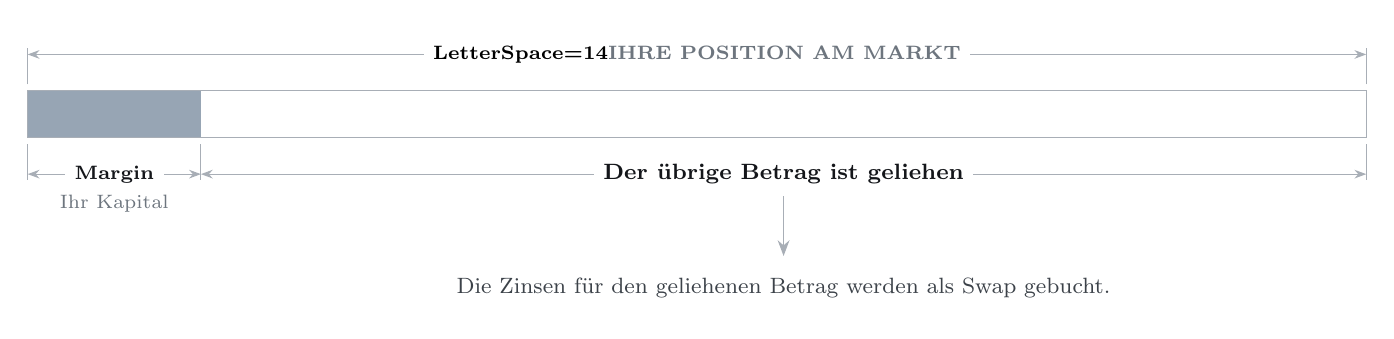
\begin{tikzpicture}[x=1mm,y=1mm]
\useasboundingbox (0,2) rectangle (170.0,38);
\fill[pfgrau] (0,24) rectangle (22.0,30);
\draw[greya,line width=0.4pt] (0,24) rectangle (170.0,30);
\draw[hilfslinie] (0,30.8) -- (0,35.4) (170,30.8) -- (170,35.4)
  (0,23.2) -- (0,18.6) (22,23.2) -- (22,18.6) (170,23.2) -- (170,18.6);
\mass{0}{170}{34.6}{\micro\bfseries\ls\color{muted}IHRE POSITION AM MARKT}
\mass{0}{22.0}{19.4}{\micro\bfseries\color{ink}Margin}
\mass{22.0}{170}{19.4}{\lbl\bfseries\color{ink}Der übrige Betrag ist geliehen}
\node[inner sep=0,text=muted,font=\micro] at (11.0,15.6) {Ihr Kapital};
\draw[greya,line width=0.5pt,-{Stealth[length=2mm]}] (96,16.6) -- (96,9);
\node[inner sep=0,text=body,font=\lbl] at (96,5) {Die Zinsen für den geliehenen Betrag werden als Swap gebucht.};
\end{tikzpicture}
\par\vspace{5mm}
\Htwo{Zusammensetzung des Swaps}
\noindent\makebox[\linewidth][c]{
\begin{tikzpicture}[x=1mm,y=1mm,
  term/.style={anchor=base west,inner sep=0,font=\hthree,text=ink},
  op/.style={anchor=base west,inner sep=0,font=\fontsize{12}{15}\selectfont,text=muted},
  klammer/.style={greya,line width=0.5pt,decorate,decoration={brace,mirror,amplitude=1.4mm}},
  notiz/.style={anchor=base,inner sep=0,font=\micro,text=muted}]
\path (0,0) (0,30);
\node[term] (a) at (0,17) {Zins am Geldmarkt};
\node[op] (p) at ([xshift=5mm]a.base east) {+};
\node[term] (b) at ([xshift=5mm]p.base east) {Aufschlag des Brokers};
\node[op] (g) at ([xshift=5mm]b.base east) {=};
\node[term] (c) at ([xshift=5mm]g.base east) {Ihr Swap};
\foreach \n in {a,b,c} \draw[klammer] ([yshift=-2.8mm]\n.base west) -- ([yshift=-2.8mm]\n.base east);
\node[notiz] at ([yshift=-8.6mm]a.base) {Zinssatz für Kredite zwischen Banken};
\node[notiz] at ([yshift=-8.6mm]b.base) {Marge des Anbieters};
\node[notiz] at ([yshift=-8.6mm]c.base) {pro Nacht gebuchter Betrag};
\end{tikzpicture}}
\par\vspace{5mm}
{\color{muted}\small\raggedright Für jedes Instrument gelten zwei Sätze: \textbf{Swap long} für Buy und \textbf{Swap short}
für Sell. In der Regel sind beide negativ; ist ein Satz positiv, wird Ihnen der Betrag gutgeschrieben.
Beide Werte finden Sie im Info-Fenster des Instruments.\par}
\hr
\Htwo{Zeitpunkt der Buchung}
\noindent 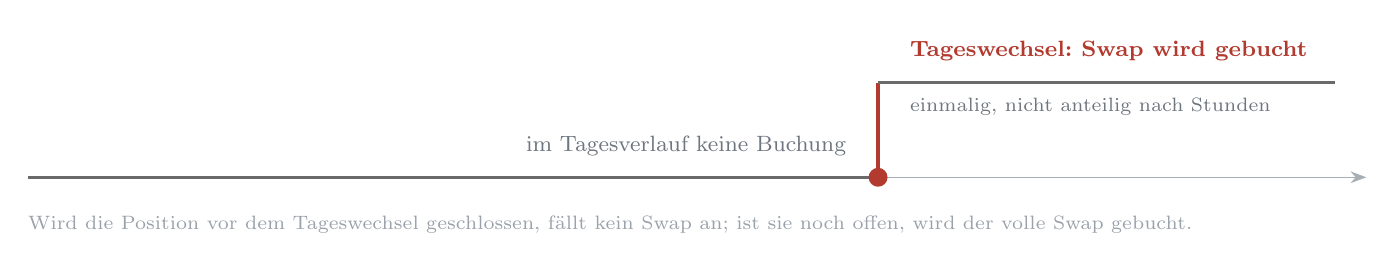
\begin{tikzpicture}[x=1mm,y=1mm]
\useasboundingbox (0,1) rectangle (170.0,29);
\draw[greya,line width=0.5pt,-{Stealth[length=2mm]}] (0,10) -- (170.0,10);
\draw[pfgrey,line width=1.2pt] (0,10) -- (108.0,10);
\draw[sell,line width=1.2pt] (108.0,10) -- (108.0,22);
\draw[pfgrey,line width=1.2pt] (108.0,22) -- (166.0,22);
\fill[sell] (108.0,10) circle (1.2);
\node[anchor=east,inner sep=0,text=muted,font=\lbl] at (104.0,14) {im Tagesverlauf keine Buchung};
\node[anchor=west,inner sep=0,text=sell,font=\lbl\bfseries] at (112.0,26) {Tageswechsel: Swap wird gebucht};
\node[anchor=west,inner sep=0,text=muted,font=\micro] at (112.0,19) {einmalig, nicht anteilig nach Stunden};
\node[anchor=west,inner sep=0,text=soft,font=\micro] at (0,4) {Wird die Position vor dem Tageswechsel geschlossen, fällt kein Swap an; ist sie noch offen, wird der volle Swap gebucht.};
\end{tikzpicture}
\par\vspace{3mm}
\noindent 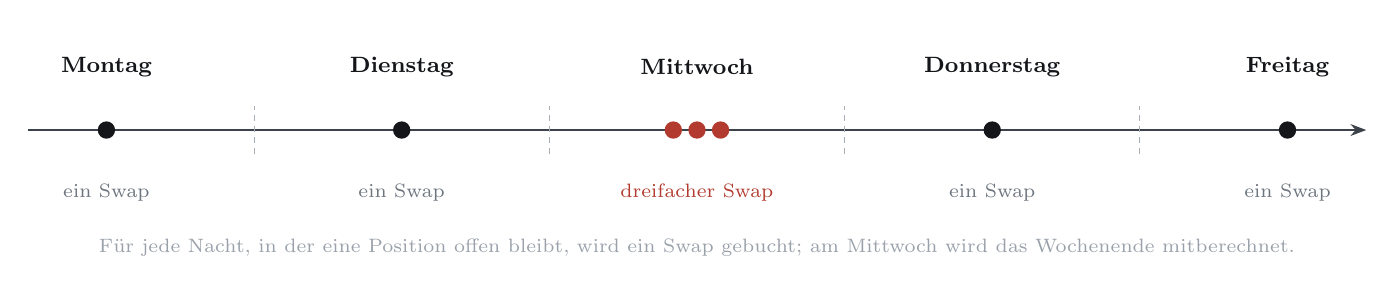
\begin{tikzpicture}[x=1mm,y=1mm]
\useasboundingbox (0,1) rectangle (170.0,31);
\draw[body,line width=0.7pt,-{Stealth[length=2mm]}] (0,18) -- (170.0,18);
\node[inner sep=0,text=ink,font=\lbl\bfseries] at (10.0,26) {Montag};
\fill[ink] (10.0,18) circle (1.1);
\node[inner sep=0,text=muted,font=\micro] at (10.0,10) {ein Swap};
\draw[greya,line width=0.4pt,dash pattern=on 0.7mm off 0.7mm] (28.75,15) -- (28.75,21);
\node[inner sep=0,text=ink,font=\lbl\bfseries] at (47.5,26) {Dienstag};
\fill[ink] (47.5,18) circle (1.1);
\node[inner sep=0,text=muted,font=\micro] at (47.5,10) {ein Swap};
\draw[greya,line width=0.4pt,dash pattern=on 0.7mm off 0.7mm] (66.25,15) -- (66.25,21);
\node[inner sep=0,text=ink,font=\lbl\bfseries] at (85.0,26) {Mittwoch};
\fill[sell] (82.0,18) circle (1.1);
\fill[sell] (85.0,18) circle (1.1);
\fill[sell] (88.0,18) circle (1.1);
\node[inner sep=0,text=sell,font=\micro] at (85.0,10) {dreifacher Swap};
\draw[greya,line width=0.4pt,dash pattern=on 0.7mm off 0.7mm] (103.75,15) -- (103.75,21);
\node[inner sep=0,text=ink,font=\lbl\bfseries] at (122.5,26) {Donnerstag};
\fill[ink] (122.5,18) circle (1.1);
\node[inner sep=0,text=muted,font=\micro] at (122.5,10) {ein Swap};
\draw[greya,line width=0.4pt,dash pattern=on 0.7mm off 0.7mm] (141.25,15) -- (141.25,21);
\node[inner sep=0,text=ink,font=\lbl\bfseries] at (160.0,26) {Freitag};
\fill[ink] (160.0,18) circle (1.1);
\node[inner sep=0,text=muted,font=\micro] at (160.0,10) {ein Swap};
\node[inner sep=0,text=soft,font=\micro] at (85.0,3) {Für jede Nacht, in der eine Position offen bleibt, wird ein Swap gebucht; am Mittwoch wird das Wochenende mitberechnet.};
\end{tikzpicture}
\par\vspace{3mm}
\begin{merk}\textbf{Zusammenfassung.} Für eine Position, die Sie am selben Tag schließen, fällt kein Swap an.
Halten Sie eine Position über mehrere Nächte, wird für jede Nacht ein Swap gebucht, am Mittwoch in dreifacher Höhe.
Der Swap wird bei jeder Position in der Spalte \textbf{Swap} ausgewiesen und ist im angezeigten Profit bereits
enthalten; er wirkt sich folglich unmittelbar auf das Ergebnis der Position aus.\end{merk}
\clearpage
\kicker{}{In der Plattform}
\Hone{Wo Sie die Werte finden}
\begin{minipage}{130mm}\lead{Die mobile Ansicht und der Desktop zeigen dieselben Werte unter denselben
Begriffen. Oben ist die mobile Kontoübersicht abgebildet, darunter die Leiste am Desktop.}\end{minipage}
\par\vspace{7mm}
% Mobile Ansicht (mobil.pdf: Kopfleiste + Reiter + panel.pdf, 440 x 516 CSS-px) im Maßstab
% des bisherigen Panels (78 mm für 452 px). Koordinaten unten in CSS-px, y nach unten.
% Marken A/B: weißer Ring/Rahmen im Bild, Linie nach rechts zur Marke in der Spalte der
% Nummern 1–5 (Mittelpunkt 86 mm, Text ab 90,6 mm wie in der Liste).
\newlength\mpx\setlength\mpx{\dimexpr78mm/452\relax}
% Kreis wie \pfn, aber als eigener Knoten (ein \tikz in einem Knoten erbt dessen Anker).
% Grundlinie des Textes 0,7ex unter der Kreismitte, wie bei \pfn in der Liste.
\newcommand\tippmarke[3]{% {y in px}{Buchstabe}{Text}
  \draw[ink,line width=0.5pt,overlay] (440,#1) -- ($(0,#1)+(82.6mm,0)$);
  \node[overlay,circle,fill=ink,text=white,inner sep=0,minimum size=4.4mm,
    font=\bfseries\fontsize{7}{8}\selectfont] at ($(0,#1)+(86mm,0)$) {#2};
  \node[overlay,anchor=base west,inner sep=0,outer sep=0,text=body]
    at ($(0,#1)+(90.6mm,-0.7ex)$) {#3};}
\noindent\begin{minipage}[t]{78mm}\vspace{0pt}\begin{tikzpicture}[x=\mpx,y={(0,-\mpx)}]
\node[anchor=north west,inner sep=0,outer sep=0] at (0,0) {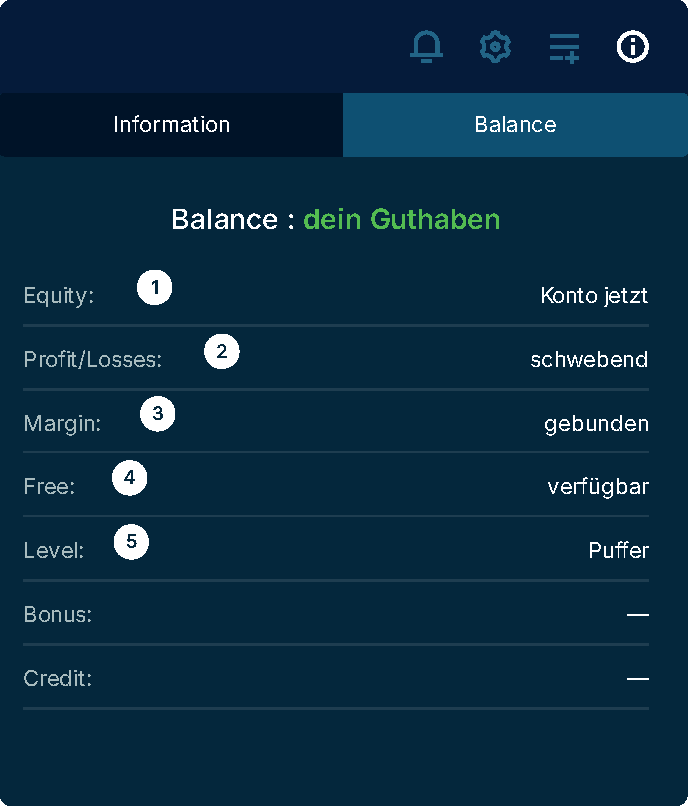
\includegraphics[width=440\mpx]{mobil.pdf}};
\draw[white,line width=1.5\mpx] (405,30) circle[radius=16] (421.75,30) -- (440,30);
\draw[white,line width=1.5\mpx,rounded corners=2\mpx] (222.75,62.75) rectangle (437.25,97.25);
\tippmarke{30}{A}{Tippen Sie oben rechts auf das {\bfseries Info-Zeichen}.}
\tippmarke{80}{B}{Tippen Sie anschließend auf {\bfseries Balance}.}
\end{tikzpicture}\end{minipage}\hfill
\begin{minipage}[t]{86mm}\vspace{1mm}\raggedright
\vspace{20mm}
\begin{enumerate}[label=\protect\pfn{\arabic*},leftmargin=6.6mm,labelsep=2.4mm,itemsep=3mm,topsep=0pt]
\item {\bfseries Equity}\newline{\color{muted}\small Der aktuelle Kontowert: Balance zuzüglich Profit/Losses.}
\item {\bfseries Profit/Losses}\newline{\color{muted}\small Das unrealisierte Ergebnis der offenen Positionen.}
\item {\bfseries Margin}\newline{\color{muted}\small Der als Sicherheit gebundene Teil der Equity.}
\item {\bfseries Free}\newline{\color{muted}\small Der für neue Positionen verfügbare Teil der Equity.}
\item {\bfseries Level}\newline{\color{muted}\small Das Verhältnis von Equity zu Margin; Maßstab für den Abstand zum Stop out.}
\end{enumerate}
\par\vspace{3mm}
{\color{soft}\small Die \textbf{Balance} steht ganz oben. Die Felder \textbf{Bonus} und \textbf{Credit}
sind für den regulären Handel ohne Bedeutung.}
\end{minipage}
\hr
\Htwo{Am Desktop: dieselben Werte in einer Zeile}
\noindent
\includegraphics[width=170mm]{bar.pdf}
\par\vspace{3mm}
{\color{soft}\small Die Leiste befindet sich unten rechts und ist dauerhaft sichtbar. Sie enthält dieselben Werte
wie die mobile Ansicht; die \textbf{Balance} steht hier am Anfang der Reihe.}
\par\vspace{7mm}
\noindent\begin{minipage}[t]{82mm}\vspace{0pt}\begin{soft}[equal height group=plattform]
{\htwo\ls\color{muted}DESKTOP}\par\vspace{2.5mm}
{\color{body}Die Kontoübersicht befindet sich in der \textbf{untersten Leiste}. Offene Positionen werden
direkt unter dem Chart angezeigt, einschließlich der Spalten \textbf{Swap} und \textbf{Commission}. Angaben
zu einem Instrument erhalten Sie über das \textbf{Info-Zeichen} in der Kursliste.}\end{soft}\end{minipage}\hfill
\begin{minipage}[t]{82mm}\vspace{0pt}\begin{soft}[equal height group=plattform]
{\htwo\ls\color{muted}MOBILE}\par\vspace{2.5mm}
{\color{body}Tippen Sie oben rechts auf das \textbf{Info-Zeichen}. Zunächst öffnet sich
\textbf{Information}; nach Antippen von \textbf{Balance} erscheint die oben abgebildete Ansicht. Der Reiter
\textbf{Information} zeigt \textbf{Leverage} und \textbf{Stop out}. Positionen finden Sie unter
\textbf{Orders} → \textbf{Active}; aufgeklappt zeigen sie Swap und Margin.}\end{soft}\end{minipage}
\clearpage
\kicker{}{Auf einen Blick}
\Hone{Die Begriffe im Überblick}
\begin{minipage}{130mm}\lead{Die folgende Übersicht nennt für jeden Begriff seine Bedeutung und die Anlässe, zu denen sich sein Wert ändert.}\end{minipage}
\par\vspace{9mm}
% Spalten im Flattersatz; 28 + 72 + 61,5 mm plus Spaltenabstände = 170 mm (vorher 0,4 mm zu breit)
\begin{tabular}{@{}>{\raggedright\arraybackslash}p{28mm}>{\raggedright\arraybackslash}p{72mm}%
  >{\raggedright\arraybackslash}p{61.5mm}@{}}
\hd{Begriff} & \hd{Bedeutung} & \hd{Änderung} \\
\addlinespace[1.6mm]\midrule\addlinespace[2.4mm]
\textbf{Balance} & Einzahlungen und Ergebnisse geschlossener Positionen & Bei Schließen, Ein- und Auszahlung sowie Swap \\ \addlinespace[2mm]
\textbf{Equity} & Balance zuzüglich Profit/Losses & Mit jeder Kursbewegung \\ \addlinespace[2mm]
\textbf{Profit/Losses} & Unrealisiertes Ergebnis der offenen Positionen & Mit jeder Kursbewegung \\ \addlinespace[2mm]
\textbf{Margin} & Als Sicherheit gebundener Teil der Equity & Beim Öffnen und Schließen von Positionen \\ \addlinespace[2mm]
\textbf{Free} & Equity abzüglich Margin & Mit jeder Kursbewegung und jeder Position \\ \addlinespace[2mm]
\textbf{Level} & Equity im Verhältnis zur Margin & Mit jeder Kursbewegung und jeder Position \\ \addlinespace[2mm]
\textbf{Leverage} & Verhältnis von Volumen zu Margin & Fest je Konto und Instrument \\ \addlinespace[2mm]
\textbf{Swap} & Zinsen für das Halten über Nacht & Jede Nacht, am Mittwoch dreifach \\
\end{tabular}
\par\vspace{6mm}
\begin{merk}\textbf{Kernaussagen.} Die Equity gibt den aktuellen Wert Ihres Kontos wieder, die Balance hingegen nur
die bereits realisierten Ergebnisse. Free bezeichnet den Teil der Equity, der für weitere Positionen zur Verfügung
steht. Der Hebel bestimmt nicht die Richtung eines Ergebnisses, sondern das Ausmaß, in dem eine Kursbewegung
auf Ihr Konto wirkt.\end{merk}

\end{document}
